\section{Overview of the EU-Structure}
\label{sec:EU-Structure}

\subsection{The structure of the EU}
Art. 1 of the present EU Treaty states: \set{\ldots} The Union shall be founded on the European Communities, supplemented by the policies and forms of cooperation established by this Treaty. \set{\ldots} Based on this provision, the image of a temple with three pillars was created:

\begin{itemize}
\item 1st pillar: the European Communities, based on the Community Treaties (today: Euratom and the European Community; the Coal and Steel Community expired in 2002); in the EU Treaty, Titles II, III and IV contain changes to the Community Treaties;
\item 2nd pillar: the Common Foreign and Security Policy (CFSP), based on Title V of the EU Treaty;
\item 3rd pillar: Police and Judicial Cooperation in Criminal Matters (PJCCM), based on Title VI of the
EU Treaty.
\end{itemize}

Under the Lisbon Treaty (Reform Treaty), Art. 1 of the Treaty on European Union (TEU) provides that the Union shall be founded on the present Treaty and on the Treaty on the Functioning of the European Union. What is now the EC Treaty is renamed Treaty on the Functioning of the European Union, and the former changes to this Treaty that at present can be found in Title II of the EU Treaty are incorporated into the Treaty on the Functioning of the European Union (TFEU). The EC no longer exists under this name but is succeeded by the European Union, which is now given explicit legal personality (Art. 47 TEU).
Further, the former changes to the Euratom Treaty that at present can be found in Title IV of the EU Treaty are incorporated into the Euratom Treaty. New changes to this Treaty can be found in Protocol No 2 to be attached to the Lisbon Treaty (OJ 2007 C 306/199). This means that the only remaining Community is formally no longer part of the EU. At the same time, Euratom is linked to the EU as certain provisions of the EU and FEU Treaties apply also to Euratom (\eg regarding the institutions).

\clearpage
\subsection{The structure of the EU and FEU Treaties}
The revised Treaties are characterised by a new structure.
The revised EU Treaty contains titles on:
\begin{enumerate}
\item Common provisions;
\item Democratic principles;
\item The institutions;
\item Enhanced cooperation;
\item The Unions external action (general provisions) and the CFSP (specific provisions);
\item Final provisions.
\end{enumerate}
The TFEU (revised and renamed EC Treaty) contains parts on:
\begin{enumerate}
\item Principles;
\item Non-discrimination and citizenship;
\item Union policies and internal actions;
\item Association of overseas countries and territories;
\item External action by the Union;
\item Institutions and the budget;
\item Final provisions.
\end{enumerate}

The above means that what at present is the 3rd pillar is to use the old term communitarised (\ie moved into what is now the 1st pillar and what in the future will be the TFEU). Only the Common Foreign and Security Policy maintains a special position on the level of the EU Treaty.

\clearpage
\subsection{A new metaphor for the EU}
The above changes beg the question as to whether the metaphor of the temple with three pillars can still be used in order to describe the set-up of the European Union. According to some, it can indeed (\eg Kiiver).1 However, it is submitted that the special position of the CFSP is really the only feature that may remind one of the pillar structure. Again, the Lisbon Treaty contains no provision that would evoke the image of three distinct pillars. Also, the fact that Euratom is detached from the EU means that the old image is no longer adequate.

Instead, the image suggested in the chapter on the Lisbon Treaty complementing Essential EC Law in Charts by Tobler/Beglinger is that of the European Union as a planet around which Euratom circles like a satellite. In fact, the picture of the planet can be taken further by representing the three legal texts of equal value that govern the European Union (namely the TEU and the TFEU as the two treaties on which the EU is founded, and, according to Art. 6(1) TEU the Charter of Fundamental Rights) as the core, the mantle and the crust of the planet (below, picture 1)

\begin{figure}[h]
\caption{EU-Structure as a planet}
\centering
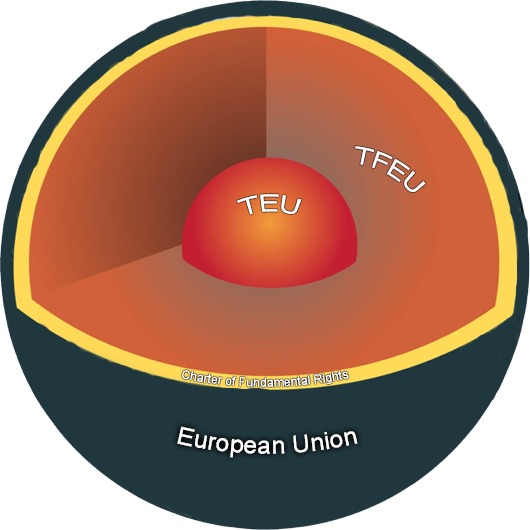
\includegraphics[width=0.4\textwidth]{images/struktur.png}
\end{figure}
\clearpage